% This is samplepaper.tex, a sample chapter demonstrating the
% LLNCS macro package for Springer Computer Science proceedings;
% Version 2.20 of 2017/10/04
%
\documentclass[runningheads]{llncs}
%
\usepackage[citestyle=numeric,style=numeric,backend=biber]{biblatex}
\usepackage{cleveref}
\usepackage{subcaption}
\usepackage{makecell}
\addbibresource{literature.bib}
\usepackage{graphicx}
\usepackage{caption} 
\captionsetup[table]{skip=10pt}
% Used for displaying a sample figure. If possible, figure files should
% be included in EPS format.
%
% If you use the hyperref package, please uncomment the following line
% to display URLs in blue roman font according to Springer's eBook style:
% \renewcommand\UrlFont{\color{blue}\rmfamily}

\begin{document}
%
\title{Machine Learning Methods for Solving Differential Equations}
%
%\titlerunning{Abbreviated paper title}
% If the paper title is too long for the running head, you can set
% an abbreviated paper title here
%
\author{Dmitrii Seletkov \\
Advisor: Vadim Arzamasov}
%
\authorrunning{Dmitrii Seletkov}
% First names are abbreviated in the running head.
% If there are more than two authors, 'et al.' is used.
%
\institute{Karlsruhe Institute of Technology, Kaiserstr. 12, 76131 Karlsruhe, Germany
\email{dmitrii.seletkov@student.kit.edu}\\
\email{vadim.arzamasov@kit.edu}}
%
\maketitle              % typeset the header of the contribution
%
\begin{abstract}
Differential equations are a ubiquitous tool for modeling the processes in physics, chemistry, finance, etc. Their numerical solution remains often challenging due to infeasible computational costs. In contrast, the application of machine learning shows great results in many related areas. This seminar work addresses current challenges in solving partial differential equations and investigates the diversity of the recent approaches that use machine learning techniques. The state-of-the-art works are explored by categorizing them into three major directions. First, theory-guided approaches that integrate the underlying physics of the process into machine learning models. Second, neural operators that directly learn a mapping between functional parameters to the solutions facilitating a high level of generalization. Third, high-dimensional approaches that mitigate the curse of dimensionality and propose effective solvers for equations with more than 100 dimensions.

\keywords{PDE \and Machine Learning \and Deep Learning}
\end{abstract}
%
%
%

\section{Introduction}
Many problems in physics, finance, engineering are described through differential equations. Differential equations provide a natural language to model processes in real world. Nowadays computers usually solve them numerically. However, traditional numerical methods require a lot of computational power and become infeasible, since it is desired to simulate complex processes precisely. Thus, applied mathematics is permanently searching for the new numerical methods or ''effective equations`` that are derived from the original differential equation, but can be solved faster with satisfactory accuracy.

On the other hand, in recent years, machine learning and, especially, deep learning have achieved great results in various areas. Therefore, these techniques have been also applied to solve the differential equations. This seminar work aims at broad investigating of the numerous approaches used to solve partial differential equations. We point out three main directions of recent work. First, theory-guided approaches that try incorporating physics prior knowledge into learning models, to make them more understandable and get rid of the black-box nature of deep learning. Second, neural operators that learn the solution operator, instead of learning of a concrete instance and, thus, promote generalization. Third, the distinct group of approaches for solving differential equations in high dimensional spaces, which notoriously suffer from the curse of dimensionality. In this work, we mainly focus on the applied machine learning techniques and not on the mathematical or physical meanings.

The remainder of this work is structured as follows. \Cref{sec:foundations} overviews the necessary fundamentals in numerical solving of partial differential equations. In \cref{sec:tga} we discuss the diversity of theory-guided approaches. In \cref{sec:neuraloperators} we present the novel neural operators applied to solve differential equation. \Cref{sec:highdim} describes the approaches for solving high-dimensional differential equations. In \cref{sec:conclusion} we summarize the conclusions of this seminar work and point out the possible direction of future works. 


\section{Foundations}
\label{sec:foundations}
A Partial Differential Equation (PDE) is a differential equation that involves partial derivatives in a function with multiple variables. Compared to ordinary differential equation (ODE), a PDE has two or more independent variables. PDEs are usually constrained by boundary and initial conditions. Boundary conditions restricts the behavior of a function on the border of its area of definition. Initial conditions are similar to boundary, but specify temporal information.  

\subsection{Partial Differential Equations Classifications}
In scientific literature, different types of classifications are used for PDEs. Large groups of equations with similar properties are identified, in order to define the common problems and suggest a general solution for them. Usually, PDEs are classified by order, homogeneity and linearity~\cite{pdesum}. Besides them, second-order and fluid equations have supplementary parameters, introduced below.

\subsubsection{Order} is a natural number that determines the highest derivative term in differential equation.

\subsubsection{Homogeneity} If all terms of a PDE contains a dependent variable or its partial derivatives, the PDE is non-homogeneous. Otherwise, the PDE is homogeneous.

\subsubsection{Linearity} A PDE is linear, if the unknown function and its derivatives appear to the power of 1, otherwise it is non-linear. Or equivalent, a PDE is linear, if the dependent variable and all its partial derivatives occur linearly, otherwise it is non-linear. A PDE is quasi-linear, if all the terms with highest order derivatives of dependent variables occur linearly that is the coefficients of such terms are functions of only lower order derivatives of the dependent variables. However, terms with lower order derivatives can occur in any manner. For instance, \cref{eq:linpde} is linear, \cref{eq:quasilinpde} and \cref{eq:nonlinpdeex} are non-linear, and \cref{eq:quasilinpde} is quasi-linear.
\begin{equation}
\frac{\partial^{2} u}{\partial t^{2}}-c^{2} \frac{\partial^{2} u}{\partial x^{2}}=0
\label{eq:linpde}
\end{equation}

\begin{equation}
u x \frac{\partial^{2} u}{\partial x^{2}}+u^{2} x y \frac{\partial^{2} u}{\partial x \partial y}+u y \frac{\partial^{2} u}{\partial y^{2}}+\left(\frac{\partial u}{\partial x}\right)^{2}+\left(\frac{\partial u}{\partial y}\right)^{2}+u^{3}=0
\label{eq:quasilinpde}
\end{equation}

\begin{equation}
\frac{\partial^{2} u}{\partial x^{2}}+\left(\frac{\partial^{2} u}{\partial x \partial y}\right)^{2}+\frac{\partial^{2} u}{\partial y^{2}}=x^{2}+y^{2}
\label{eq:nonlinpdeex}
\end{equation}

\subsubsection{Elliptic, parabolic and hyperbolic} Since many physical laws are described by the second-order PDEs, they are additionally classified into elliptic, parabolic and hyperbolic~\cite{pdevideo}. Given a PDE:
\begin{equation}
A \frac{\partial^{2} u}{\partial x^{2}}+B \frac{\partial^{2} u}{\partial x \partial y}+C \frac{\partial^{2} u}{\partial y^{2}}+D=0
\label{eq:pde}
\end{equation}
where $A, B, C$ are functions from $x, y$, and $D$ is a function from $x, y, t, \frac{\partial u}{\partial x}, \frac{\partial u}{\partial y}$. \Cref{eq:pde} is elliptic, parabolic or hyperbolic, when $B^2 - 4AC$ is $< 0$, $= 0$, or $> 0$, respectively.

\subsubsection{Boundary Conditions} can be two types: Dirichlet --- value of unknown function given e.g. surfaces held at fixed temperatures; or Neumann --- value of derivatives given e.g. heat flux across the boundaries.

\subsubsection{Reynolds Numbers} The PDEs describing fluid mechanics use the dimensionless parameter, called Reynolds Number~\cite{reynoldsnumber2}. A low Reynolds number ($< 2000$) indicates a laminar (sheet-like) flow, while a high Reynolds number --- turbulent flow~\cite{reynoldsnumber}.

\subsubsection{Specific Partial Differential Equations}
Some specific PDEs are named by the scientists who discovered them. The list of the PDEs used in this report and their descriptions are shown in \cref{table:pdes}.

\begin{table}
%\setlength{\tabcolsep}{20pt}
\renewcommand{\arraystretch}{1.75}
\centering
\begin{tabular}{|l|l|l|l|}
\hline
Name & Type & Description & References\\
\hline
Advection & hyperbolic & \makecell[l]{acoustic; motion of a scalar as it is advected \\ by a known velocity field} & \cite{Brenner20}\\
Allen--Cahn & parabolic & \makecell[l]{reaction-diffusion; phase separation in multi-\\component alloy systems} & \cite{Han18, Weinan17, Raissi19, Raissi1, Raissi2}\\
Black--Scholes & parabolic & \makecell[l]{finance; dynamics of a financial pricing \\ containing derivative investment instruments} & \cite{Han18, Weinan17}\\
Burgers & hyperbolic & \makecell[l]{fluid mechanics, nonlinear acoustics, gas dynamics \\ and traffic flow} & \cite{Li20, Sirignano18, Brenner19}\\
Free-boundary & parabolic & finance; determining American options & \cite{Sirignano18} \\
Hamilton--Jacobi & parabolic & \makecell[l]{dynamic programming, optimal control theory,\\ game theory} & \cite{Sirignano18, Han18, Weinan17} \\
Korteweg–De Vries & hyperbolic & \makecell[l]{behavior of waves in shallow water} &  \cite{Brenner19, Raissi19, Raissi1, Raissi2} \\
\makecell[l]{Kuramoto–\\Sivashinsky} & parabolic & \makecell[l]{reaction-diffusion; instabilities in laminar flame fronts, \\ phase dynamics in reaction-diffusion systems} & \cite{Brenner19}\\
Navier--Stokes & parabolic & \makecell[l]{fluid mechanics; motion of fluid substances\\defined by viscosity} & \cite{Li20, Raissi19, Raissi1, Raissi2, Brenner21, Ranade20, Gao21}\\
Poisson & elliptic & \makecell[l]{theoretical physics; potential field caused by \\ a given electric charge or mass density distribution} & \cite{Gao21}\\
Schrödinger & parabolic & \makecell[l]{quantum mechanics; governs the wave function\\ of a quantum-mechanical system} & \cite{Raissi19, Raissi1, Raissi2}\\
\hline
\end{tabular}
\caption{Specific Partial Differential Equations, their type, description, and references used in this report.}
\label{table:pdes}
\end{table}

\begin{figure}
	\centering
	 \begin{subfigure}{.33\textwidth}
      \centering
      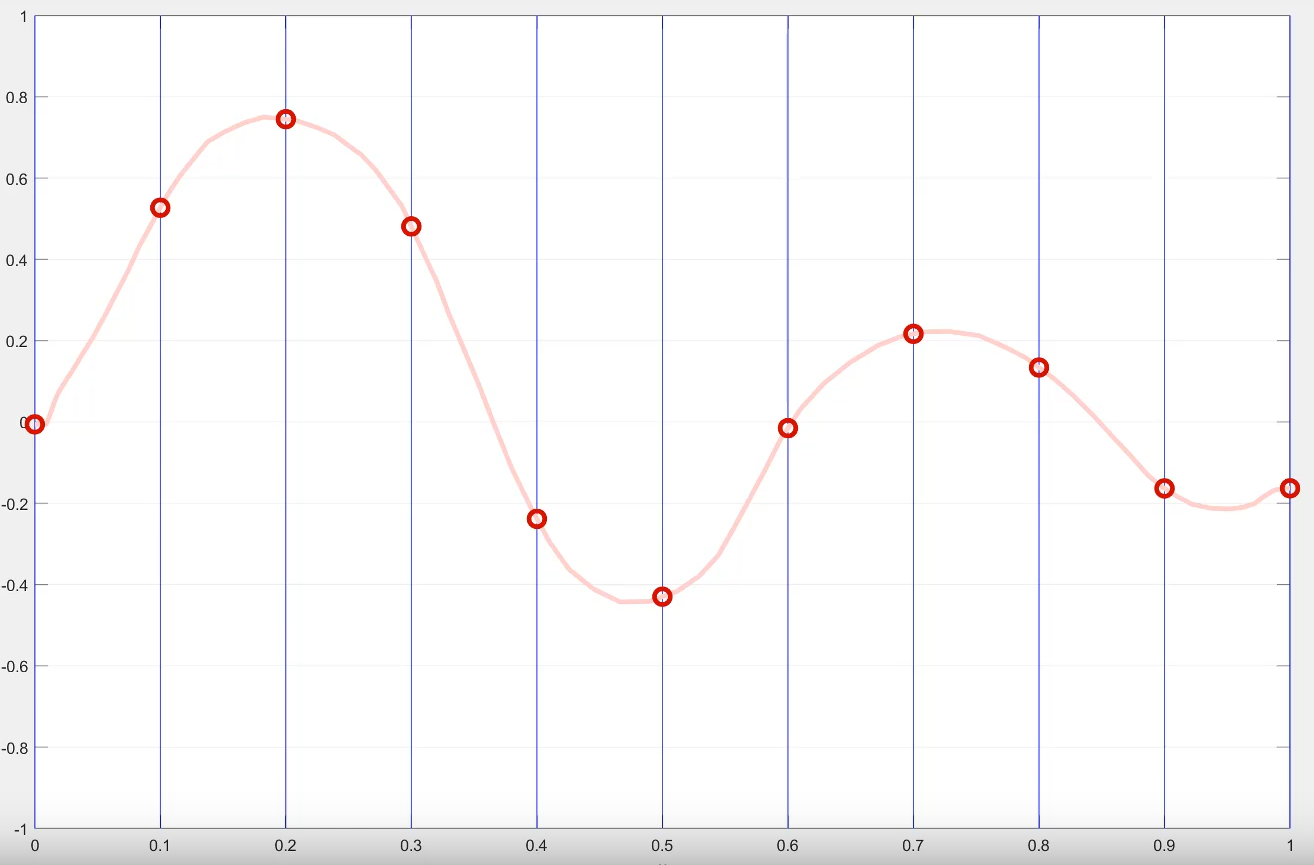
\includegraphics[width=0.99\linewidth]{figures/fdm.png}
      \caption{Finite difference}
      \label{fig:fdm}
    \end{subfigure}%
     \begin{subfigure}{.33\textwidth}
      \centering
      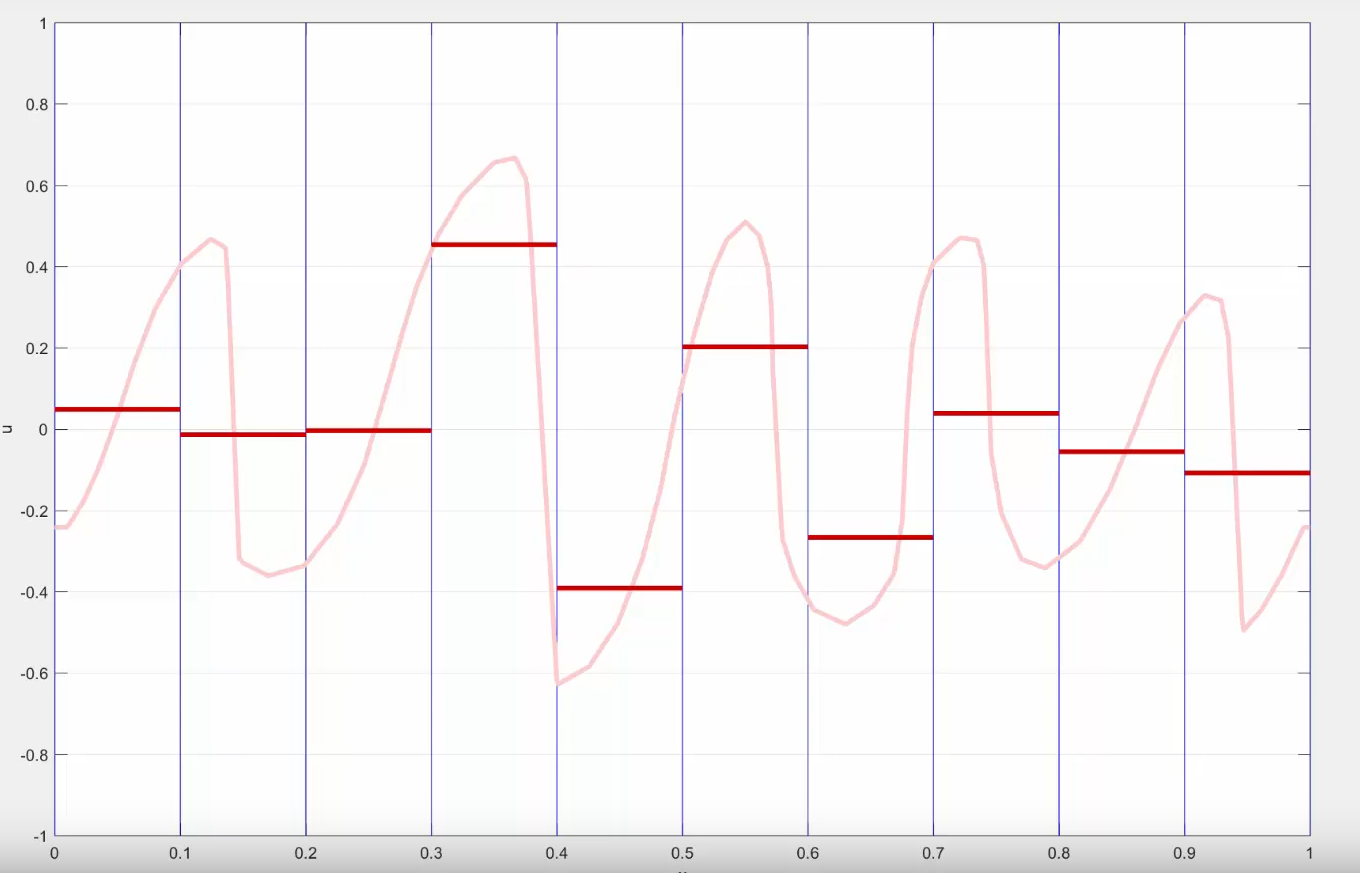
\includegraphics[width=.99\linewidth]{figures/fvm.png}
      \caption{Finite volume}
      \label{fig:fvm}
    \end{subfigure}%
	 	 \begin{subfigure}{.33\textwidth}
      \centering
      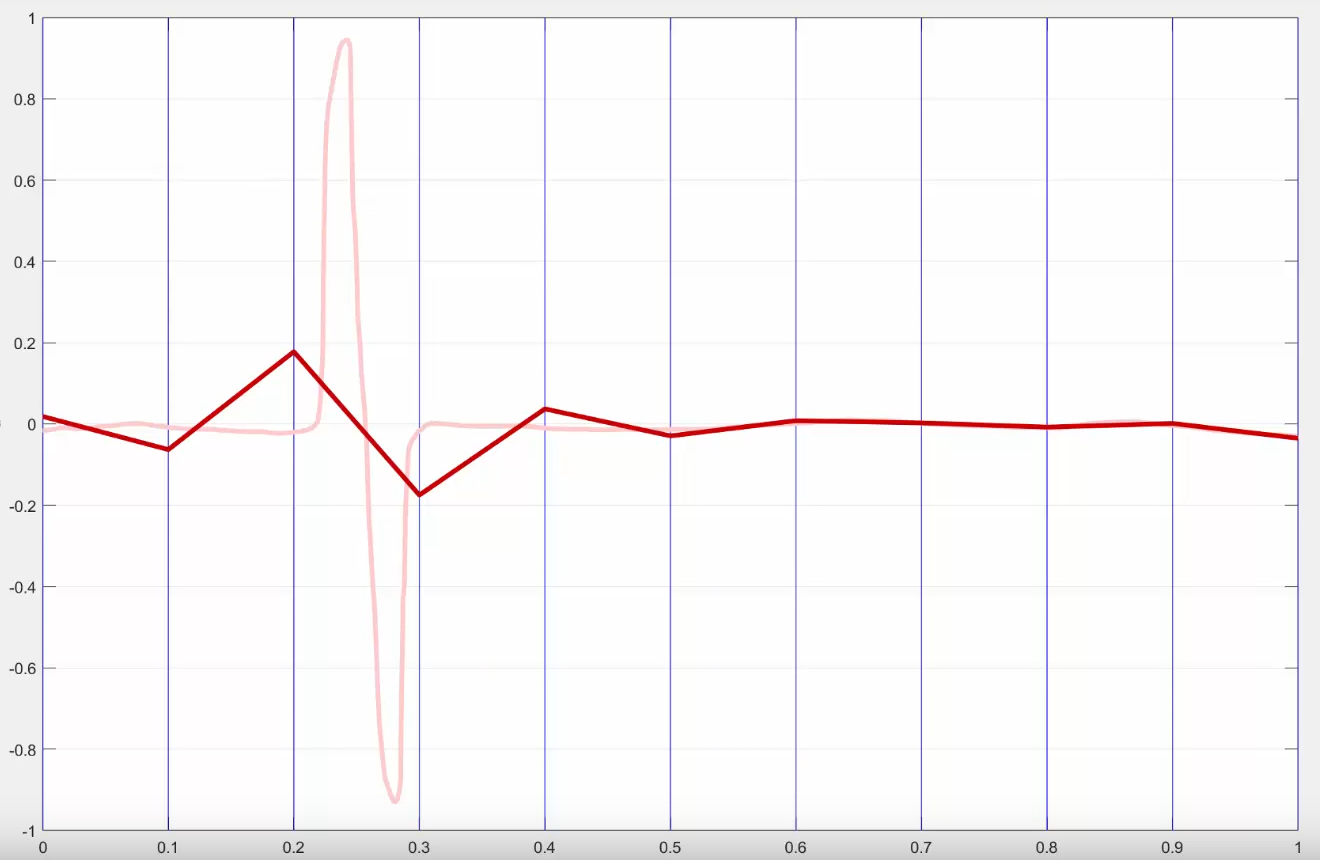
\includegraphics[width=.99\linewidth]{figures/fem.png}
      \caption{Finite element}
      \label{fig:fem}
    \end{subfigure}
	\caption{Comparison of numerical solution methods for partial differential equation: (a) finite difference (b) finite volume (c) finite element~\cite{pdesolution}.}
	\label{fig:pdesolution}
\end{figure}  

\subsection{Traditional Numerical Methods}
In numerical analysis, three common solution methods for PDEs exist: finite difference, finite volume and finite elements~\cite{pdesolution}. All of them approximate the arbitrary function using a finite number of discrete quantities. But the approximated quantities differ. The graphic comparison of these methods is shown in \cref{fig:pdesolution}.

\subsubsection{Finite Difference Method (FDM)} stores the values of the function of grid points. This is applied, when the computational costs have to be low.
\subsubsection{Finite Volumes Method (FVM)} stores the average values between the grid points. This is applied, when the conservation property is required e.g. energy equations. 
\subsubsection{Finite Element Methos (FEM)} chooses the best approximation within the finite dimension of possible basis functions (elements). FEM is the most flexible, but computational intensive compared to FDM and FVM.


%\subsection{Machine Learning Basics}
\section{Theory-guided Approaches}
\label{sec:tga}
Partial Differential Equations (PDE) has often to be solved in physics. Thus, besides the observational data from experiments, the underlying equations that describes the physics of the process are also known. The approaches that use not only pure data, but also integrate the underlying physics of the process into the machine learning models are called theory-guided~\cite{tgds} or physics-informed~\cite{Raissi19}. 

Theory-guided approaches can be further classified by their source, representation and integration~\cite{inltax}; or more detailed into Basic ML, Physics-Guided
Loss Function, Physics-Guided Initialization, Physics-Guided Architecture, Residual Model and Hybrid Model~\cite{survey}. Other ways to classify the theory-guided PDE Solvers are the applied numeric scheme (finite difference, finite volume or finite element-based) or type of equation (elliptic, parabolic, hyperbolic).

Since in the recent works the diverse combinations from the different categories are applied, we use in the following subsections the classification from Gao et al.~\cite{Gao21} into continuous and discrete.


\subsection{Continuous Approaches}
Continuous physics-informed approaches are a baseline for many physical problems. They commonly employ the fully-connected neural network architecture. Continuous approaches use point-wise automatic differentiation technique~\cite{ad} to compute space and time derivatives and approximate the continuous solution of PDE with respect to given coordinates. 

\subsubsection{Physics-informed Neural Networks (PINNs)}
Similar approaches existed earlier~\cite{similarPINN}, but Raissi et al.~\cite{Raissi19, Raissi1, Raissi2} have first formulated them as a new paradigm --- Physics-Informed Neural Networks (PINNs) --- to solve all types of PDEs. 

Most supervised machine learning approaches require much data and do not take into account physical laws and, thus, usually fail when applied to a limited amount of data. To mitigate this problem, the prior knowledge defined by physical equation induces the loss function of the trained network. This acts as a regularizer and restricts the solution space incorporating the PDE.

Raissi et al.~\cite{Raissi19} investigate two major problems: data-driven solution~\cite{Raissi1} and data-driven discovery~\cite{Raissi2} of PDEs. In these works, they use simple fully-connected (FC) feed-forward networks without additional regularization, and hyperbolic tangent activation function. The method was evaluated on Schrödinger, Allen--Cahn, Korteq--de Vries and Navier--Stokes equations and showed promising results. 

\subsubsection{Diversity of approaches}
The proposed by Raissi et al. method is applied to many scientific areas: nano-optics~\cite{nanooptics}, elastodynamics~\cite{elastodynamics}, diagnosing atrial fibrillation  ~\cite{fibrillation}. Moreover, NVIDIA created a SimNet framework based on continuous physics-informed approaches to assist in solving physics problems on their GPUs~\cite{nvidia}.

Despite the broad application of continuous PINNs, all of them have similar limitations. First, continuous approaches have high computational training costs. Second, integrating of proper initial and boundary condition for more than 2-D spaces in PDE requires hard ad hoc designing~\cite{Gao21}. Therefore, describing constraints for more complicated real-world PDEs remains challenging using continuous approaches. Third, the theoretical error and convergence estimations are absent in the model. Thus, employing Bayesian optimization~\cite{sno12} is a part of the future works.

Finally, the authors point out that the proposed method is not a replacements of exiting numerical methods, but a supplement for hybrid models to enhance the quality and and reduce the computational cost of predictions. Moreover, the questions e.g. about depth and structure of the model, amount of needed data, possibility of vanishing and exploding gradients, etc. remain uninvestigated. 


\subsection{Discrete Approaches}
Discrete physics-informed approaches have reduced computational costs and better scalability compared to continuous ones. They commonly employ convolutional neural network (CNN) architecture. Discrete approaches use automatic differentiation technique~\cite{ad} to learn space and time solutions directly based on numerical discretization scheme.

\subsubsection{Data-driven Discretization}
Typical pipeline for solving PDEs consists of three main steps. First, we take a PDE that simulates a physical process e.g. Burgers equation $\frac{\partial v}{\partial t}+v \frac{\partial v}{\partial x}=\eta \frac{\partial^{2} v}{\partial x^{2}}$. Second, discretize it in space and represent on the mesh e.g. $\quad \frac{\partial^{2} v}{\partial x^{2}} \approx \frac{v_{i+1}-2 v_{i}+v_{i-1}}{\Delta x^{2}}$. This results in a large set of ODEs that can be solved numerically. If we want to understand what happens in simulation e.g. weather simulation, $\Delta x$ must be small, whereby the number of mesh points must be large. 

Numerical solutions of a PDE is difficult. Therefore, applied mathematics tries to derive an effective equation that can be solved numerically with lower computational power. This analytical process is usually ad hoc and difficult~\cite{brennerLecture}. To mitigate it, Bar--Sinai et al.~\cite{Brenner19} propose a Data-driven Discretization method.

All solutions of PDEs are in infinite dimensions, but the solutions for a concrete PDE instance are in low-dimensional manifold~\cite{titi89}. Therefore, the main idea is to parameterize solution manifold and execute machine learning model to obtain it. Hence, for a given PDE:
\begin{equation}
    \begin{array}{l}\frac{\partial v}{\partial t}=\mathcal{L}(t, x, v, \nabla v, \nabla \nabla v, \ldots) \end{array}
    \label{eq:ddd1}
\end{equation}
Discretize in finite differences and approximate with weights and mesh points:
\begin{equation}
    \begin{array}{l}\quad \frac{\partial^{n} v}{\partial x^{n}}|_{x_{i}+\frac{\Delta x}{2}} \approx \sum_{k=-N}^{N} \alpha_{k}^{(n)} \hat{v}_{i+k} \end{array}
    \label{eq:ddd2}
\end{equation}
Classical approaches derive weights from calculus, but in this approach ${\alpha}_{k}^{(n)}$ is learned instead. Intuitively, it helps to learn how the solutions look like based on data, instead of performing direct interpolation. For example, the comparison between polynomial and neural net interpolation is shown in \cref{fig:ddi}.

\begin{figure}
	\centering
	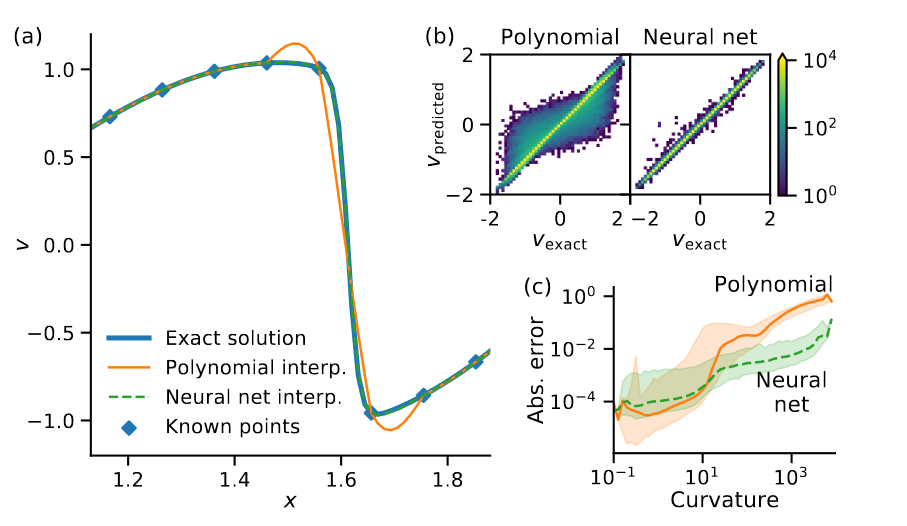
\includegraphics[width=10cm]{figures/ddinterpolation.png}
	\caption{Comparison between polynomial and neural net interpolation. Intuition: instead of performing direct polynomial interpolation, learn the solution manifold based on data, i.e. how the solutions look like~\cite{Brenner19}.}
	\label{fig:ddi}
\end{figure}  

The method Data-driven Discretization consists of three steps: perform many high-resolution simulations, train a regressor algorithm to machine learn the solution manifold and use it to estimate spatial derivatives from low-resolution data and integrate over them.

The method was evaluated on Burgers, Kuramoto--Sivashinsky and Korteweg--de Vries equations. The authors achieved remarkably accurate results for one-dimensional problems with 4-8 times coarser discretization resolution compared to standard finite difference methods.

This approach suffers from two major limitations. First, CNN requires more computational operations than finite difference implementation. This results in problems with inference speed. Second, the method was mainly evaluated in one dimension, while real-world problems have usually two or more dimensions.

To address this issue, Kochkov et al.~\cite{Brenner20} investigate Data-driven Discretization in the following work and adjust it for two-dimensional problems. 

Both training and inference are shown in \cref{fig:ddd}. First steps do not differ from the original Data-driven discretization. The CNN learns to predict finite difference coefficients in the spatial derivatives. Then, finite volume scheme is used to compute time derivatives, as performed in the numerical method of lines~\cite{schiesser91}. In contrast to the previous method, the results are accumulated over 10 timestamps to minimize the difference between model predictions and ground truths from high-resolution simulations. Multi-step mean absolute error (MAE) loss function is employed. Furthermore, in contrast to the previous method, physical constraints are employed before and after neural net. To guarantee stability, normalization of input features is applied. The entire program is written in automatic differentiation framework TensorFlow to enable training a neural net inside the classical numerical solver.

\begin{figure}
	\centering
	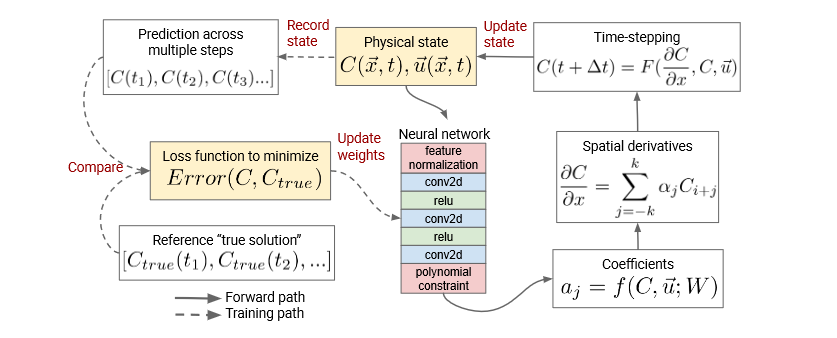
\includegraphics[width=12cm]{figures/ddd.png}
	\caption{Data-driven Discretization Framework~\cite{Brenner20}.}
	\label{fig:ddd}
\end{figure}  

Evaluated on 2-D Advection PDE, the adjusted Data-driven Discretization showed the same accuracy as the state-of-the-art numerical solver by 4 times coarser resolution in all dimensions. However, the model fails when trying to predict for predicting longer time period that it was trained. 

In order to correctly predict for out of training distribution inputs, Kochkov et al.~\cite{Brenner21} present a novel type of machine learning solvers based on Data-driven Discretization. 

The idea is to take classical state-of-the-art numerical solvers: direct numerical simulation (DNS) and large eddy simulation (LES). Replace error-prone parts such as discretization and closure affected by loss of resolution with machine learning alternatives in DNS and LES, respectively. 

Kochkov et al. propose two approaches. Learned Interpolation (LI) that replaces polynomial interpolation without prior knowledge in DES, as shown in the previous works~\cite{Brenner19, Brenner20}. And Learned Correction (LC) that models a residual correction to the discretization in LES. The principle distinction between these methods is shown in \cref{fig:lilc}. LI employs CNN architecture, while LC uses ResNet. 

Both approaches were evaluated on challenging Navier-Stokes Equation in 2D. They do not suffer from the lack of generalization compared to the predecessor. Moreover, they show the same accuracy as baseline solvers with 8-10 times coarser resolution in each dimension and 40-80 times computational speed-up. Thus, the recent approach has solved the problems encountered in the first versions of Data-driven Discretization solvers.

The evolution of the approaches based on Data-driven Discretization show another possibility to embed the physical constraints into PDE solvers. Compared to the classical PINNs, which mainly apply ``soft'' constraints in form of the loss function, these approaches apply ``hard'' constraints. They replace only some components of numerical solvers with neural nets and, hence, can impose the physical constraints before and after machine learning solvers per construction. This type of synergy improves the existing solvers and guarantees physical consistency at the same time.

\begin{figure}
	\centering
	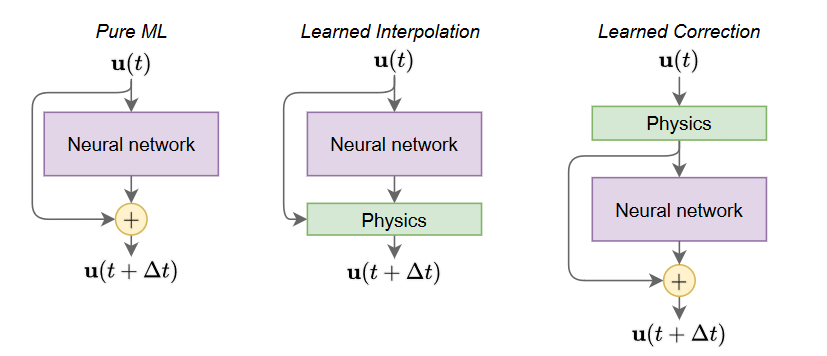
\includegraphics[width=12cm]{figures/lilc.png}
	\caption{The principle difference between Pure ML methods and proposed Learned Interpolation and  Learned Correction is in position of applied physics constraints~\cite{Brenner21}.}
	\label{fig:lilc}
\end{figure}  


\subsubsection{Data-free Discretization}

Data-driven approaches often require large data-sets obtained by high-cost computational simulations on supercomputers. To resolve this problem a series of works investigate the data-free approaches.

These approaches use neural networks to generate data constrained by physical loss in spirit of classical PINNs and iteratively learn to enhance the solutions as performed in numerical solvers.

Ranade et al. propose a DiscretizationNet~\cite{Ranade20}. This ML-Solver comprises a finite volume based discretization scheme in neural network within the automatic differentiable computational graph. Neural network employs a generative encoder-decoder CNN architecture and is shown in \cref{fig:discretizationnet}. Inputs consist from flow variables, boundary condition encoding and geometry encoding. First, the encoder encodes the inputs in lower dimensional latent vector. The latent vector is extended with boundary condition and geometry encoding to enrich the latent space. Second, the latent vector is decoded. Outputs are inserted as inputs into the network again. The iterative process continues until the determined time or reached accuracy. In the training process the physical loss is incorporated in spirit of classical PINNs.

Compared to traditional computational fluid dynamics (CFD) solver ANSYS, the proposed method shows better performance and training stability for three steady Navier--Stokes cases: lid-driven cavity, laminar flow past cylinder and conjugate heat transfer. In future works, the ML-Solver can be investigated for unsteady problems by extending with LSTMs and for other types of PDEs with more complex physics.

\begin{figure}
	\centering
	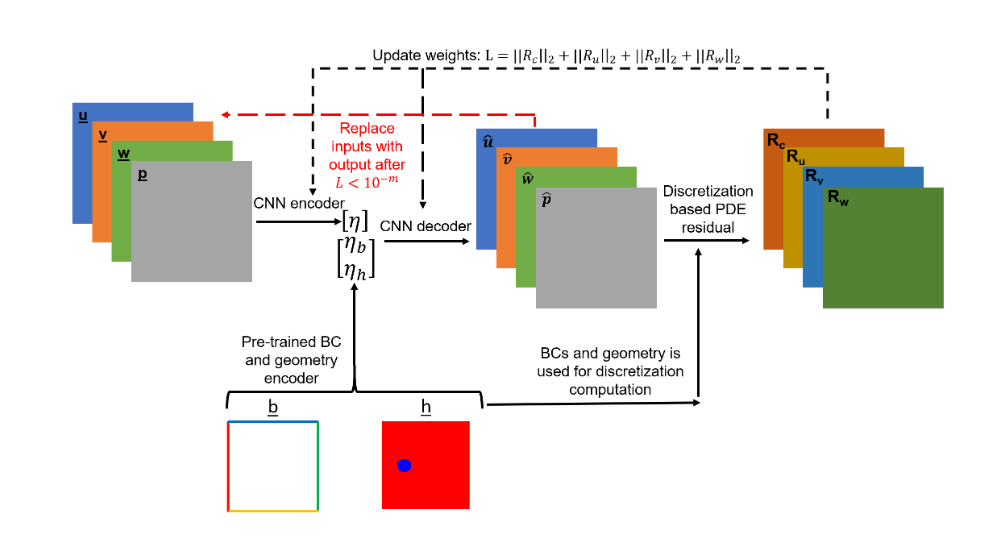
\includegraphics[width=12cm]{figures/discretizationnet.png}
	\caption{Architecture DiscretizationNet for Navier--Stokes Equation. This employs a generative encoder-decoder CNN for data-free PDE learning~\cite{Ranade20}.}
	\label{fig:discretizationnet}
\end{figure}  

\subsubsection{Finite element based Discretization}

The aforementioned works apply finite difference or finite volume schemes. Since the finite element scheme is more accurate for numerous tasks, Yao et al. propose a FEA-Net~\cite{feanet}. This is a discrete PINN based on FEM that employs CNN architecture. The special FE-based convolution is introduced to calculate PDE residuals in physics-informed loss. Due to convolutional backbone the methods are limited to rectangular domains and cannot model irregular geometries with unstructured meshes, so as all CNN-based networks. Since the Fully-connected architecture also suffers from problems such as scalability and incorporation of hard boundary conditions, Gao et al.~\cite{Gao21} propose a novel framework that is based on FEM and employs Graph Convolutional Networks (GCN).

The proposed method has three main features. First, in the input vector of GCN, each spatial coordinate of the mesh has its own node. After forward propagation, GCN outputs the graph with discretized solution fields, where each solution vector is in a separate node. This structure does not require rasterization and allows to internally handle unstructured mesh with simplex quadrilateral elements in spirit of classical FEM solver. Second, Gao et al. apply piece-wise polynomial basis functions that help to make predictions based on output graph. This decreases the search space dimension to improve PDE-informed convergence. Third, the essential boundary conditions are enforced by construction. Therefore, no tuning of penalty coefficient is required. 

Evaluated on Poisson and steady Navier--Stokes problems, the proposed method mitigates the problems caused by FC and CNN architectures and shows the effectiveness and robustness against them. The authors point out the use of combination of deep learning and numerical methods rather than their separation in future works, in order to improve generalability and achieve better results.

\section{Neural Operators}
\label{sec:neuraloperators}
The universal approximation theorem~\cite{universalT} says that a neural network can approximate an arbitrary continuous function. This fact is exploited widely in the current deep learning research in computer vision, natural language procession, etc. Another important corollary from the universal approximation theorem states that a neural network can also approximate any non-linear continuous functional or operator.

Recently, a new series of works~\cite{deeponet, bhattacharya21, nelsen21, Li20} explore the idea to create a neural operator for solving PDEs. 

Neural operator learns to parameterize a mapping between function spaces instead of learning a mapping between finite-dimensional Euclidean spaces as the classical neural networks do. For PDEs the neural operator learns a mapping between functional parameters to the solutions. This has many advantages compared to classical neural network approaches discussed in \cref{sec:tga}. Neural operator is mesh-independent, since it can transfer the solutions between meshes and used for different discretization. Once neural operator learned, it can be applied to different instances in the whole family of PDE. Furthermore, neural operator does not require the underlying PDE, but only data. 

The recent works can be classified into two categories: approaches that use Euclidean function spaces and those that use Fourier function spaces. 

\subsection{Euclidean Space Operator}
Most of recent works \cite{deeponet, bhattacharya21, nelsen21} focus on defining operators in Euclidean space. Lu et al.~\cite{deeponet} propose a DeepONet --- the first work in this direction. 

This network approximates both linear and non-linear operators from a restricted amount of data, instead of approximating functions. This inputs infinite dimensional functions and outputs other functions but in output space. As shown in \cref{fig:deeponet}, DeepONet comprises two parts: branch and trunk nets. Branch net encodes the discrete input functions at fixed sensors. Trunk net encodes the domain of the output functions. The theoretically proposed architecture is Stacked DeepONet, where branch net is executed $p$ times. In practice, the hyperparameter $p$ is high. In order to reduce computational costs, all branch networks are merged into single branch network.

The proposed method was evaluated on Gravity Pendulum ODE and Diffusion-reaction system. This shows better generalization compared to classical numerical and neural networks approaches. In future works the Li et al. intend to investigate the theoretical network size needed for the neural operator and its connection to generalization error. Moreover, other types of neural network architectures such as CNN, RNN and Transformers can be employed. 

\begin{figure}
	\centering
	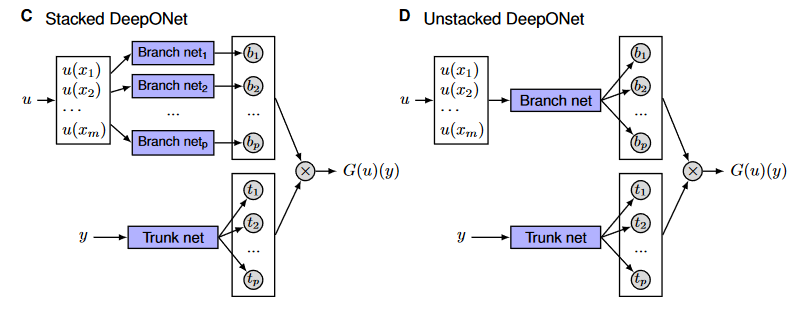
\includegraphics[width=12cm]{figures/deeponet.png}
	\caption{DeepONet comprises two parts: branch net for encoding input functions and trunk net for encoding locations for the output functions~\cite{deeponet}.}
	\label{fig:deeponet}
\end{figure}  

\subsection{Fourier Space Operator}
Differentiation in Euclidean is equivalent to multiplication in Fourier space\cite{diffequimult}. Some hybrid approaches of spectral methods and neural networks exploit this fact for solving PDEs~\cite{fan19, jiang20}. This enhances performance and precision of results, since Fourier space is more suitable for many types of PDEs~\cite{fan19}. Based on these methods, Li et al.~\cite{Li20} introduce a novel fully neural net based Fourier Neural Operator. 

This method was applied to model turbulent flow in 2D, in order to predict how initial vorticity (a curl of velocity that determines the rotational flow in the region) evolves over time. 

\subsubsection{Formal Problem Setting}
In traditional neural net solvers, we input data points with spatial and temporal coordinates $(x, y, t)$, execute the model and receive the solutions as changed with time other data points. In this approach, we input functions $a$ and receive functions $u$ of form mapping $a, u: x, y, t \mapsto vorticity$. Therefore, to solve the PDE we need to determine an operator $G_{\theta}$ with model parameters $\theta$ for input $\mathcal{A}$ and output $\mathcal{U}$ function spaces.
\begin{equation}
G_{\theta}: \mathcal{A} \rightarrow \mathcal{U}, \quad \theta \in \Theta
    \label{eq:fno}
\end{equation}

Due to using function spaces instead of data points, we do not sample on particular resolution. Thus, once functions are learned, any solution resolution is possible. 

\subsubsection{Method}
\label{fno:method}
The pipeline is shown in \cref{fig:fno}(a) and contains two main phases: up- ($P$) and down-projection ($Q$) at the beginning and end, and Fourier Neural Operator (FNO). Up-projection transforms initial state $a(x)$ into latent space. This is implemented with Conv$1\times1$ layer that takes an input tensor described by the sequence of initial timestamps (usually $t=0,...,10$). Afterwards, series of Fourier layers are executed. Finally, down-projection transforms the resulting tensor into output space. The output tensor $u(x)$ contains a sequence of predictions for many timestamps at once (usually $t=11,...,50$). FNO is shown in \cref{fig:fno}(b) and described with \cref{eq:fno1}:

\begin{equation}
v_{t+1}(x):=\sigma\left(W v_{t}(x)+\left(\mathcal{K}(a ; \phi) v_{t}\right)(x)\right)
\label{eq:fno1}
\end{equation}

where $\sigma$ is a non-linearity, $W$ is a weight matrix and $\mathcal{K}$ is a Kernel integral operator that is theoretically described with \cref{eq:fno2}:

\begin{equation}
\left(\mathcal{K}(a ; \phi) v_{t}\right)(x):=\int_{D} \kappa(x, y, a(x), a(y) ; \phi) v_{t}(y) \mathrm{d} y
\label{eq:fno2}
\end{equation}

However, the calculation of $\mathcal{K}$ causes a large computational overhead and is not possible in practice. Lu et al. propose many engineering decisions that simplifies the calculation of $\mathcal{K}$. The main idea is transformation into Fourier space $\mathcal{F}$ where we can use a plain multiplication $R$ instead of calculating convolving integral and back transformation $\mathcal{F}^{-1}$ at the end. This results in \cref{eq:fno3}:

\begin{equation}
\left(\mathcal{K}(\phi) v_{t}\right)(x)=\mathcal{F}^{-1}\left(R_{\phi} \cdot\left(\mathcal{F} v_{t}\right)\right)(x)
\label{eq:fno3}
\end{equation}

\begin{figure}
	\centering
	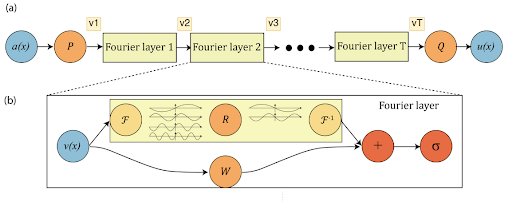
\includegraphics[width=12cm]{figures/fno.png}
	\caption{(a) Pipeline proposed by Li et al.~\cite{Li20} contains two main phases: up- ($P$) and down-projection ($Q$) and Fourier Layers. (b) Fourier Layer contains Fourier forward ($\mathcal{F}$) and back ($\mathcal{F}^{-1}$) transformation and linear multiplication ($R$) equivalent to convolution in Euclidean space.}
	\label{fig:fno}
\end{figure}  

\subsubsection{Results}
The proposed method was evaluated on Burgers, Darcy Flow and Navier--Stokes PDEs. This outperformed all existing learning-based methods in both accuracy and computation time. This is the first method that achieved zero-shot super-resolution for modelling turbulent flows. 

Fourier Neural Operator was mainly applied to modelling turbulent flows, where Fourier spaces were used earlier as a natural approach for this type of problems. Therefore, it remains under discussion, whether FNO can be applied to other PDEs.

Other limitations are related to the Method in \cref{fno:method}. First, the input consists of ten timestamps that have to be computed by either a numerical method or another ML technique. Second, it remains uninvestigated if the super-resolution is bounded and whether the output prediction can be extended to more timestamps at once, i.e. from predefined $t=11,...,50$ to e.g. $t=11,...,200$ or more.




\section{High-dimensional Approaches}
\label{sec:highdim}
In some spheres of physics, finance, chemistry it is required to solve PDEs, which number of dimensions can exceed conventional three dimensions and can reach e.g. 100 or more. These problems have to be considered separately, since they suffer from the curse of dimensionality. 

The curse of dimensionality is a group of problems that occur only in high-dimensional spaces. For example, concentration of norms and distances, instability of neighborhood, changing behavior in distribution of data, empty space phenomenon, etc. When the dimensionality increases in PDEs, computational cost for solving them grows exponentially~\cite{bellman}. 

Both numerical and machine learning approaches become infeasible in high-dimensional spaces e.g. due to the exploding number of grid points in FDM or an exponential growth of the complexity of non-linear regression models. But the combination of them can be a key toward an effective and accurate solver. 

\subsection{Reformulation as Backward Stochastic Differential Equations}
In order to use the power of deep learning, Han et al.~\cite{Han18, Weinan17} propose a deep BSDE solver, where PDEs is reformulated as Backward Stochastic Differential Equations (BSDEs) and then solved with reinforcement learning (RL). 

The method contains three steps. Firstly, a concrete PDE is reformulated as BSDE using Feyman-Kac formula that is used by solving linear parabolic PDEs numerically with Monte Carlo method. Since the BSDE is similar to stochastic control problem, model-based RL is applied to this with a gradient of solutions as a policy function. Finally, the policy function is approximated with DNN as performed in RL. The architecture of the applied DNN contains four fully-connected layers and depends on the dimensionality, but not on the type of solving PDE. Furthermore, the increasing of number of hidden layers enhances accuracy of the solver, but affects computational cost negatively. The optimal number is chosen experimentally. Batch Normalization and Adam optimizer are used.  

Tested on Black--Scholes, Hamilton--Jacobi and Allen--Cahn PDEs with up to 100 dimensions, the method achieves successful results in terms of accuracy and computational cost. Therefore, while numerical methods fail due to the curse of dimensionality, the proposed algorithm effectively includes more dependencies into equations to receive more precise results e.g. considering more economic agents, instead of using less representative agents in Black--Scholes PDE. However, the method is restricted to the class of non-linear parabolic PDEs and requires an ad hoc reformulation for each type of PDE.     

\subsection{Deep Galerkin Method}
Since meshes become infeasible in high-dimensional spaces, Sirignano et al.~\cite{Sirignano18} propose a first completely mesh-free algorithm for solving high-\\dimensional PDEs, called Deep Galerkin Method. 

Galerkin method is a numerical method that searches for a linear combination of basis functions to find the solution for a underlying PDE. Instead of a linear combination of basis function, Deep Galerkin Method approximates solutions using DNN completely mesh-free. The proposed method consists of 4 steps. First, random spatial points with fixed probability density are sampled. This allows to avoid forming a mesh. Second, squared error at these points is computed after the executing on DNN. Third, the gradients are backpropagated through DNN after taking a learning step with a fixed learning rate. Fourth, the method is repeated until the convergence. The applied DNN employs LSTM architecture with Xavier initialization. For the training L2-regularization and Adam optimizer are used. 

The method is evaluated on free-boundary pricing American options, Hamilton--Jacobi and Burgers PDEs. This achieves the accurate results with up to 200 dimensions. Although the proposed method is applied to quasi-linear parabolic PDEs, it can be extended to elliptic and hyperbolic ones. However, the performance for these types of PDE is not investigated. The authors prove the theoretical convergence of DNN to PDE solutions only for quasi-linear equations and not for the whole non-linear class of PDEs.


\section{Conclusion}
\label{sec:conclusion}
In this seminar work, we report about the diversity of the approaches that apply different machine learning techniques to solve differential equations. We point out three main categories: theory-guided to include physics knowledge into machine learning models, neural operators to improve their generalizability, and high-dimensional approaches to get rid of the curse of dimensionality. 

We observe that the plethora of techniques introduced in other spheres of computer science such as fully-connected NN, CNN, RNN, LSTMs, Transformers, etc., have found their application in mathematics to solve differential equations more accurately and effectively. Moreover, the state-of-the-art works attempt to mitigate black-box machine learning models usually based only on data by incorporating physical laws or knowledge of the underlying equation. Furthermore, the current models tend to be hybrid and use both numerical and machine learning methods for better performance and generalization. Another direction of research is searching for a universal neural differential operator that generalizes the whole differential operator in the equation and allows resolution and boundary condition independent solutions.

Based on exploration of state-of-the-art approaches, we assume that the further direction of future works can be focused on improving the generalizability by solving differential equations. This can be achieved by theory-guided hybrid models that can replace the computationally intensive parts of numerical solvers with faster neural networks. Another interesting direction of future works can be the discovering of the universal neural operators for large groups of equations. 



%
% ---- Bibliography ----
%
% BibTeX users should specify bibliography style 'splncs04'.
% References will then be sorted and formatted in the correct style.
%
% \bibliographystyle{splncs04}
% \bibliography{mybibliography}
%
\printbibliography

\end{document}
